%%%%%%% SOFTWARE NODES %%%%%%
\addcontentsline{toc}{subsection}{Software nodes}
\subsection*{Software nodes}

The processing needed to provide all the functionality is divided in nodes. Here they are presented, ordered using the data work-flow, beginning the ones using the raw input data to the system and finishing with the ones that deliver the output of the system. 
\\

\begin{itemize}
	\item{\textbf{\large Converter}}\\
This node is the first step of the code. It transforms the input data from the pi\_tracker package into the custom message used within the software. The information provided by that third-party code contains the position in the space of each joint of the body. The converter node takes only both hand's position. 
\\

It use case diagram of the node can be seen in the diagram below: 

\begin{figure}[h]
	\begin{center}
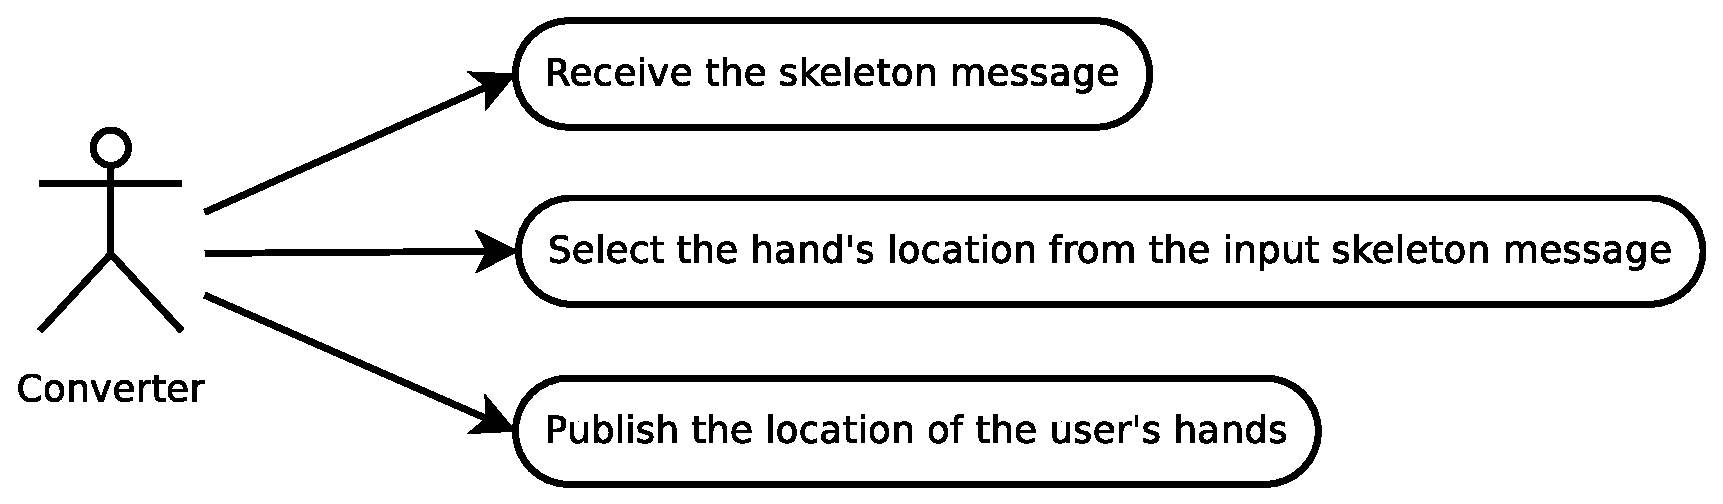
\includegraphics[scale=0.2]{img/diagrams/uc_converter.eps}
	\caption[Use case diagram converter node]{Use Case diagram of the converter node}
	\end{center}
\end{figure}

	
	\item{\textbf{ROI Segmenter 3D}}\\
The input of this node is the raw 3D information from the sensor and the hand's locations from the third-party package pi\_tracker, as well as the hand in which the user is holding the object. The node segments a prism from the original point cloud around the selected hand's center. The prism vertices coordinates are transformed from world coordinates to pixels. That information is the output of the node, together with the segmented point cloud. 

\begin{figure}[h]
	\begin{center}
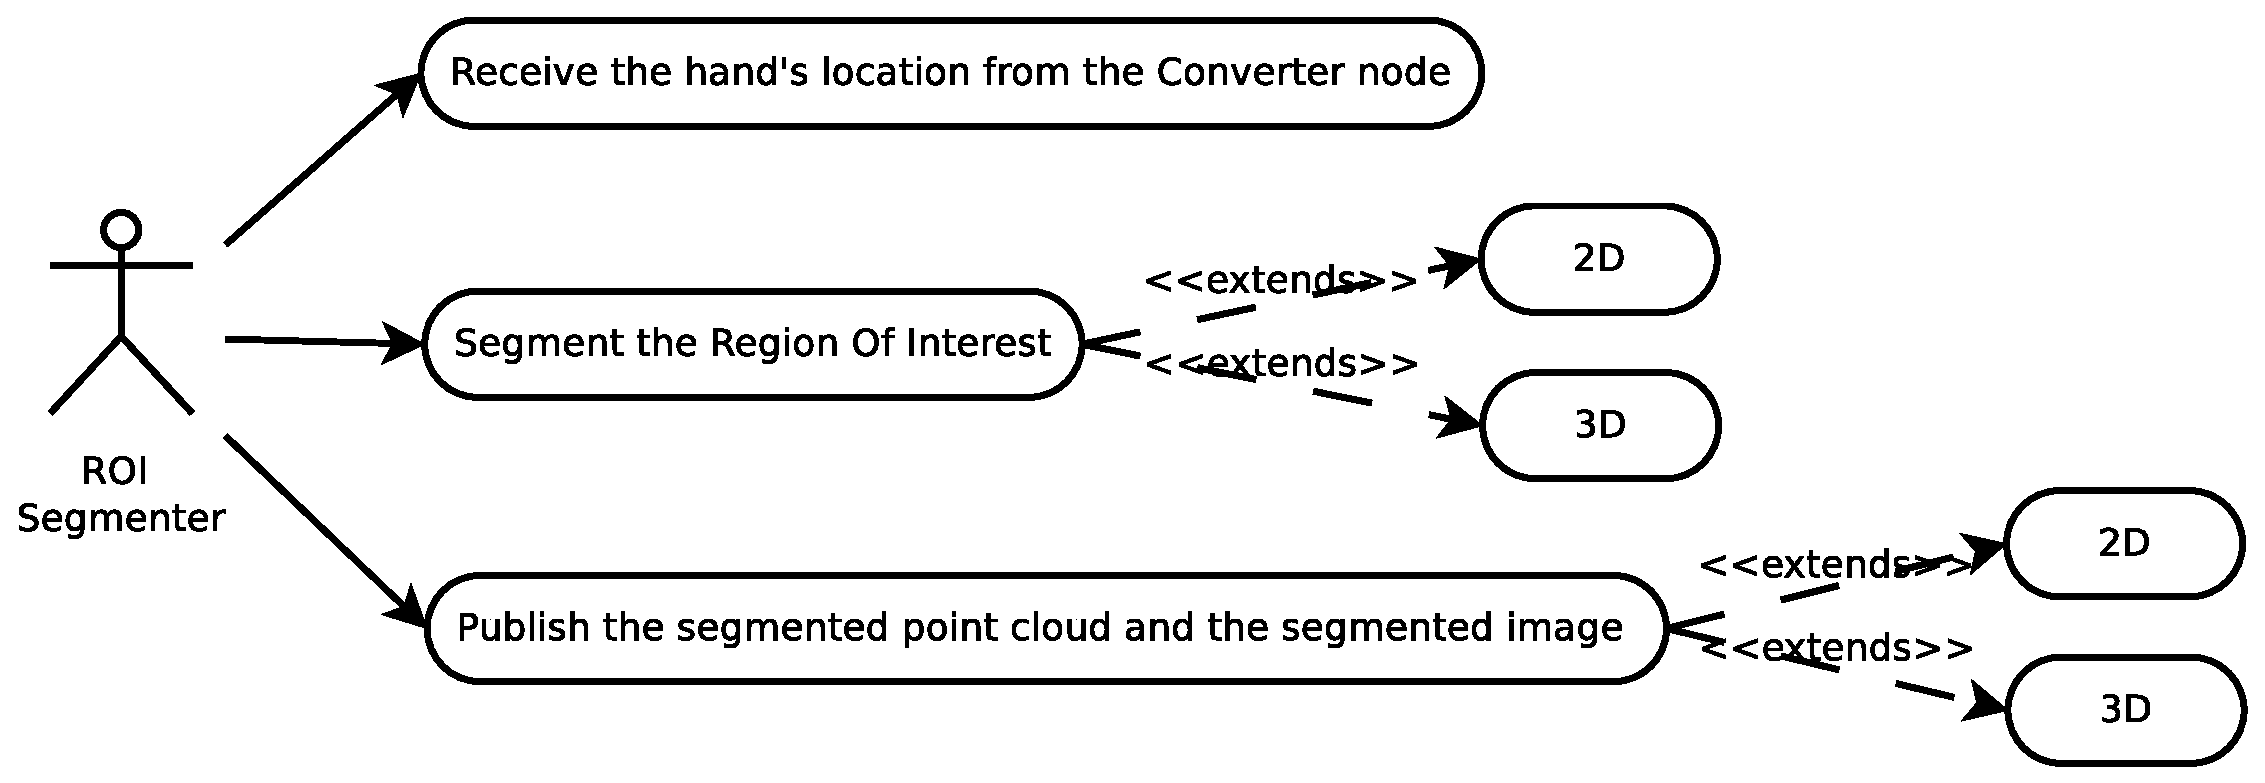
\includegraphics[scale=0.2]{img/diagrams/uc_roi_segmenter.eps}
	\caption[Use case diagram ROI segmenter 3D node]{Use Case diagram of the ROI segmenter 3D node}
	\end{center}
\end{figure}
 
	\item{\textbf{ROI Segmenter 2D}}\\
The present node takes as the input the raw 2D information from the RGB-D sensor and the hand's locations in pixels returned from the ROI segmenter 3D node. Then, it extracts the ROI (Region Of Interest) taking a square section around the center of the hand. The size of that figure is fixed for simplicity. Since due to the RGB-D sensor's current resolutions the user must remain at a fixed distance from the sensor, the difference in the scale due to the distance is negligible and hence the size can be fixed. 
\\

In the picture the use case diagram of the node can be observed.
\begin{figure}[h]
	\begin{center}
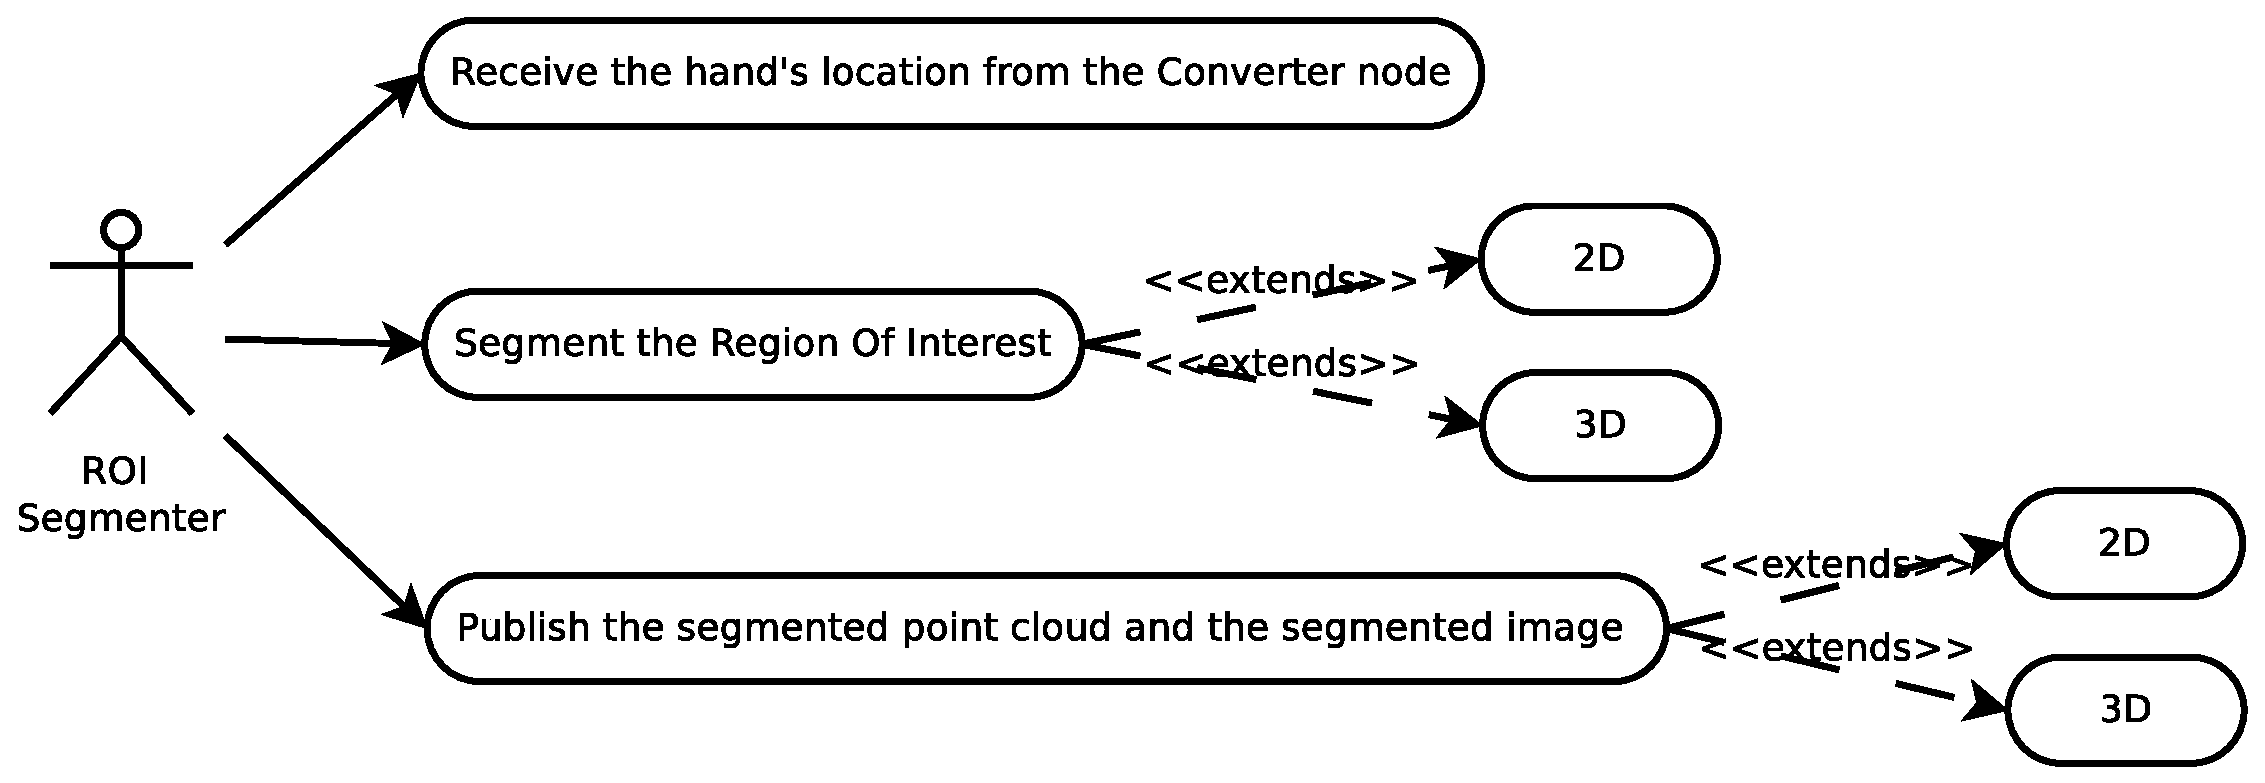
\includegraphics[scale=0.2]{img/diagrams/uc_roi_segmenter.eps}
	\caption[Use case diagram ROI segmenter 2D node]{Use Case diagram of the ROI segmenter 2D node}
	\end{center}
\end{figure}


	\item{\textbf{Feature Extractor 2D}}\\
This node takes as an input the segmented 2D ROI from the previous nodes and extracts the features. A feature is defined depending on the application and context of the computer vision project. In general, it is an interesting or important characteristic, point or region of an image. The application will determine which feature describes better the object of study. 
\\

The best feature or descriptor is that which has a higher repeatability, i.e the ability of obtaining the same output given different inputs. This is useful when making a feature matching to compare two object, which is the case in this project. 
\\

Hence, it can be seen that the recognition algorithm has as a bottle neck in its performance the repeatability of the features used to describe the different objects. 


	\item{\textbf{Feature Extractor 3D}}\\
	\item{\textbf{Event Handler}}\\
	\item{\textbf{Learner Recognizer}}\\
\end{itemize}
